% Figure M9-Tabula-Muris interp hero: interpretability-first companion.
% Generated by experiments/m9_tabula_muris.py --interpretability.
\begin{figure}[t]
 \centering
 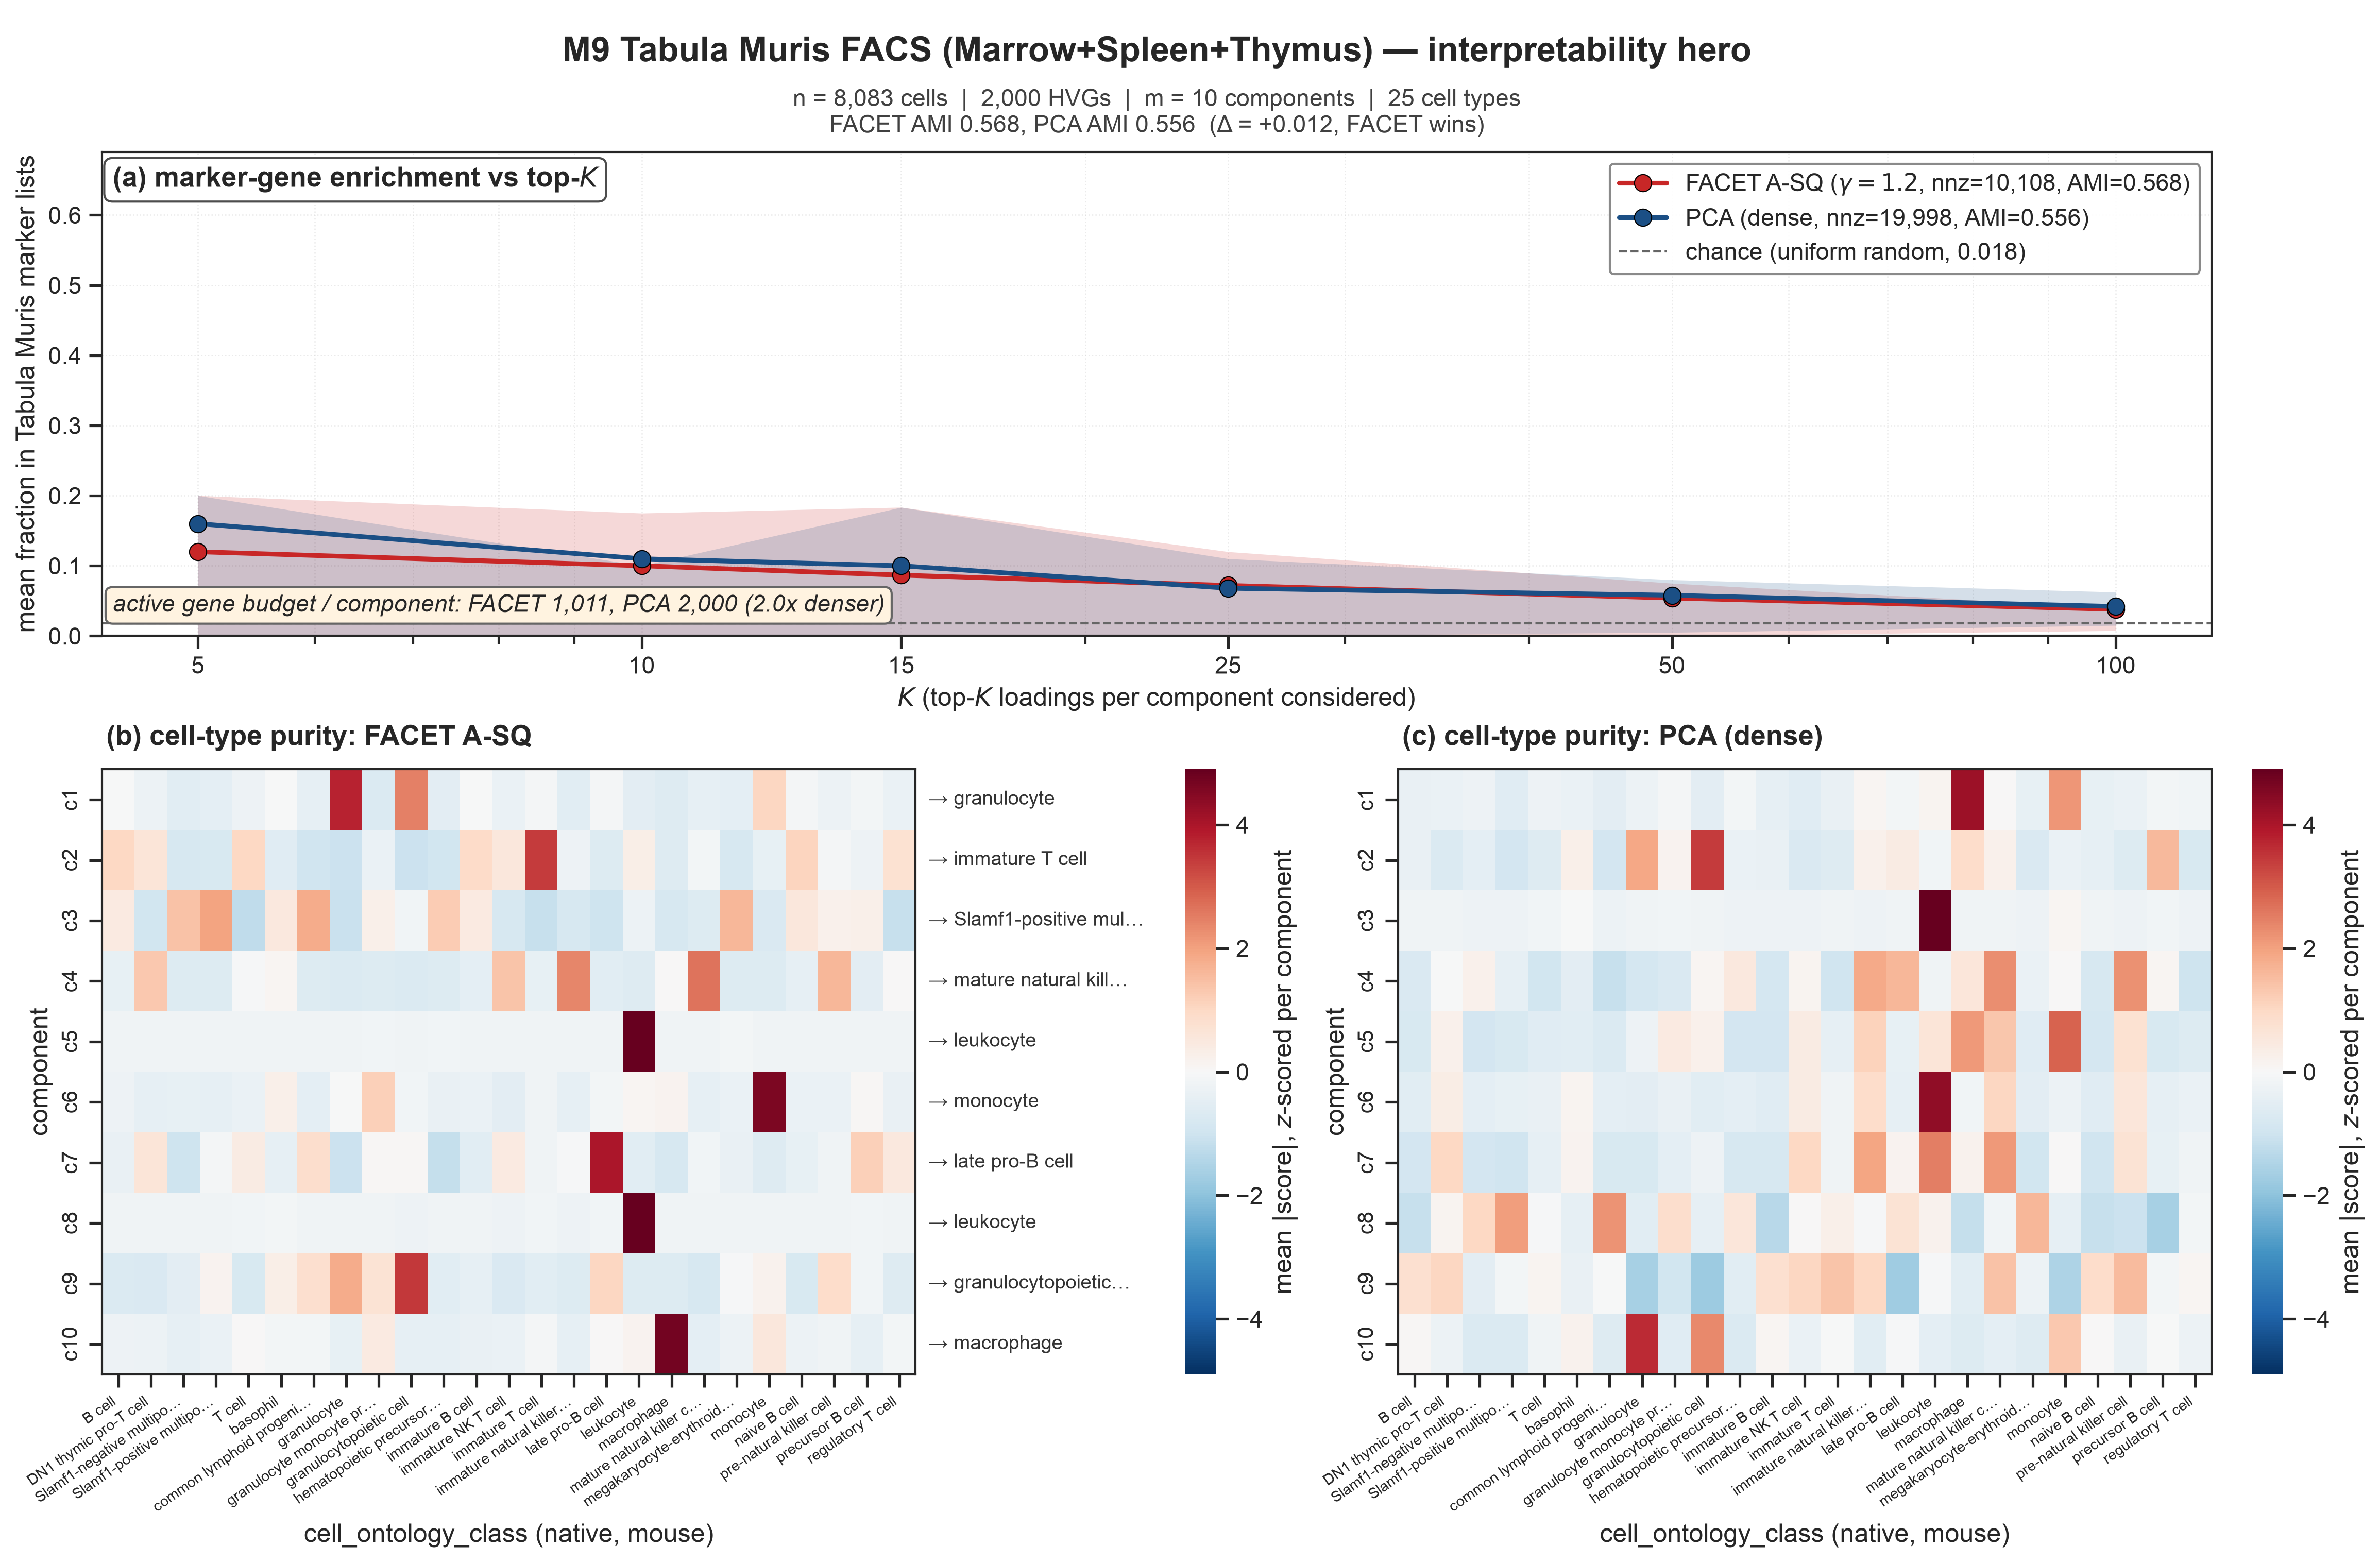
\includegraphics[width=\linewidth]{../shared/figures/generated/m9_tabula_muris_interpretability_hero.png}
 \caption{\textbf{M9 Tabula Muris interpretability hero.} Companion to Fig.~\ref{fig:m9-tabula-muris-hero}, interpretability-first panels on the same mouse Smart-seq2 data. \textbf{(a)}~Mean enrichment vs top-$K$ in the mouse immune / stromal marker list; gene-economy annotation reports per-method active-gene budget per component. \textbf{(b)}~FACET cell-type purity heatmap with dominant \texttt{cell\_ontology\_class} annotated per row. \textbf{(c)}~PCA cell-type purity on the same colour scale.}
 \label{fig:m9-tabula-muris-interp}
\end{figure}
